% TEX compiler = lualatex (Verifique no Menu se está habilitado) %
%
%----------------Escolha uma dos estilos abaixo------------------%
%%%%%%%%%%%%%%%%%%%%%%%%%%%%%%%%%%%%%%%%%%%%%%%%%%%%%%%%%%%%%%%%%%
\documentclass[Portugues,Final]{comandos} % relatorio
%\documentclass[Portugues,Final,TwoSide]{comandos} % livro
%%%%%%%%%%%%%%%%%%%%%%%%%%%%%%%%%%%%%%%%%%%%%%%%%%%%%%%%%%%%%%%%%%
%                 Dúvidas acima? Leia abaixo:
% - Primeiramente, escolha: Portugues ou Ingles ou Espanhol.
% - Para a versão final do texto, acrescente a palavra "Final":
%\documentclass[Ingles,Final]{configuracoes}

% - Há dois modos de impressão configurados, Oneside - para impresso
% estilo relatório (ou pdf para visualização na web ou computador),
%e o estilo TwoSide - apropriado para impressão como um livro.

% - Para uma compilação mais rápida, utilize a opção "Draft":
%\documentclass[Portugues,Draft]{configuracoes}

% - Adicione também a opção "noFig" para gerar arquivos mais leves:
%\documentclass[Portugues,Draft,noFig]{configuracoes}

% - Para gerar uma avaliacao antiplagio pelo Turnitin:
%\documentclass[Portugues,Final,Turnitin]{configuracoes}

%%%%%%%%%%%%%%%%%%%%%%%%%%%%%%%%%%%%%%%%%%%%%%%%%%%%%%%%%%%%%%%%%%
% Configurações gerais do documento: (não edite)
\addbibresource{bibliografia.bib}
\setlength{\headheight}{14.5pt}

\usetikzlibrary{calc}

% Estilização dos Títulos de Capítulo e Apêndice:
\titleformat{\chapter}[display]
  {\normalfont\LARGE\bfseries}
  {\fontSourceSans\bfseries\color{dtecs_titulo_azul}\LARGE\chaptertitlename~\thechapter}
  {-10pt}
  {\huge}

% Definições para ficha catalográfica
\makeatletter
\StrBefore{\@autor}{ }[\@autorprenome]
\StrBehind{\@autor}{ }[\@autorsobrenome]
\makeatother

% Definições do glossário
\loadglsentries{Elementos/glossario}

%%%%%%%%%%%%%%%%%%%%%%%%%%%%%%%%%%%%%%%%%%%%%%%%%%%%%%%%%%%%%%%%%%
%            Preencha os dados na sequência abaixo:
%%%%%%%%%%%%%%%%%%%%%%%%%%%%%%%%%%%%%%%%%%%%%%%%%%%%%%%%%%%%%%%%%%
\begin{document} 
% Escolha entre autor ou autora:
\autor{Nome do autor}
%\autora{Nome da Autora}

% Comandos para a ficha catalográfica (formato ABNT)
\autorprenome{Prenome do autor}
\autorsobrenome{Ultimo Nome}
% O mesmo para o orientador:
\orientadorprenome{Nome Completo do}
\orientadorsobrenome{Orientador}

% Sempre deve haver um título em português:
\titulo{Título da Dissertação ou Tese em Português}
\subtitulo{Subtítulo da Dissertação ou Tese} % Se houver

% Se a língua for o inglês ou o espanhol defina:
%\title{The Dissertation or Thesis Title in English or Spanish}

% --- PALAVRAS-CHAVE ---
\palavraschave{Palavra1}{Palavra2}{Palavra3} %----ESCREVA AQUI----%

% Escolha entre orientador ou orientadora e inclua os títulos:
\orientador{Prof. Dr. Nome do Orientador}
%\orientadora{Profa. Dra. Nome da Orientadora}

% Escolha entre coorientador ou coorientadora, se houver:
%\coorientador{Prof. Dr. Eng. Lic. Nome do Co-Orientador}
%\coorientadora{Prof. Dra. Eng. Lic. Nome da Co-Orientadora}

% Escolha entre uma das seis opções a seguir (comente as demais):
%\tcc                   % para Trabalho de Conclusão de Curso.
%\qualificacaoMestrado  % Para textos de qualificação de mestrado.
%\qualificacaoDoutorado % Para textos de qualificação de doutorado.
\mestrado               % para Dissertação de Mestrado.
%\doutorado             % para Tese de Doutorado.

%Defina a área de concentração. Se for TCC, deixe comentado.
\areaConcentracao{Desenvolvimento e Sociedade}
%\areaConcentracao{Desenvolvimento e Tecnologias}

% Se houve cotutela, defina:
%\cotutela{Universidade XXX}

% Defina a data da defesa no formato {Dia}{Mês}{Ano}
% Use apenas números! O template transformará em palavras,
% se necessário.
\datadadefesa{25}{7}{2025} % ----------IMPORTANTE------------ %

% Para a versão final defina:
% Repita o nome do Orientador(a) no primeiro avaliador
\avaliadorA{Prof. Dr. Nome do Orientador}{PPG-DTECS/UNIFEI}
\avaliadorB{Profa. Dra. Segunda Avaliadora}{Instituição da segunda avaliadora}
\avaliadorC{Dr. Terceiro Avaliador}{Instituição do terceiro avaliador}
% \avaliadorD{Prof. Dr. Quarto Avaliador}{Instituição do quarto avaliador}
% \avaliadorE{Prof. Dr. Quinto Avaliador}{Instituição do quinto avaliador}
% \avaliadorF{Prof. Dr. Quinto Avaliador}{Instituição do sexto avaliador}

% Descomente na versão final, caso prefira anexar a ficha de um PDF:
%\fichaCatalografica{SeuArquivo.pdf}

% Para deixar uma página em branco no lugar da ficha 
% catalográfica, descomente uma das três linhas a seguir:
%\fichaCatalografica{branco.pdf} % Português
%\fichaCatalografica{white.pdf}  % Inglês
%\fichaCatalografica{blanco.pdf} % Espanhol

% Descomente a linha abaixo se seu trabalho tiver ilustrações
\newif\ifhasillustrations\hasillustrationstrue 

%%%%%%%%%%%%%%%%%%%%%%%%%%%%%%%%%%%%%%%%%%%%%%%%%%%%%%%%%%%%%%%%%%
% --- Inicio das páginas pré-textuais  ---
%%%%%%%%%%%%%%%%%%%%%%%%%%%%%%%%%%%%%%%%%%%%%%%%%%%%%%%%%%%%%%%%%%

% (Não edite aqui. Em caso de erros, entre em contato com o PPG)
\paginasiniciais
  \pagestyle{empty} % páginas pré-textuais sem cabeçalho/rodapé
  \setlength{\oldparindent}{\parindent}
  \setlength\parindent{0pt}
  \makeatletter
  \let\ps@mystyle\ps@plain
  \let\ps@plain\ps@empty
  \hypersetup{
    pdfcreator   = {Criado com o modelo para teses e dissertações do PPG-DTECS, elaborado por Matheus Mendonça dos Reis, Ms.},
    pdftitle     = {\@titulo},
    pdfauthor    = {\if\@autora\relax\@autor\else\@autora\fi},
    pdfsubject   = {\@monopt\xspace apresentada ao Programa de Pós-Graduação em Desenvolvimento, Tecnologias e Sociedade da Universidade Federal de Itajubá como parte dos requisitos para a obtenção do título de \@degnamept\xspace.}
}
\label{pretextual-end}
%%%%%%%%%%%%%%%%%%%%%%%%%%%%%%%%%%%%%%%%%%%%%%%%%%%%%%%%%%%%%%%%%%
% --- Fim das páginas pré-textuais / Início das textuais ---
%%%%%%%%%%%%%%%%%%%%%%%%%%%%%%%%%%%%%%%%%%%%%%%%%%%%%%%%%%%%%%%%%%

% (Não edite aqui. Em caso de erros, entre em contato com o PPG)
\fimdaspaginasiniciais{
  \cleardoublepage
  \makeatletter
  \let\ps@plain\ps@mystyle
  \makeatother
  % Definição das primeiras páginas dos capítulos
  \fancypagestyle{plain}{
    \fancyhf{}
    \fancyhead[R]{\thepage}
    \renewcommand{\headrulewidth}{0pt}
    \renewcommand{\headheight}{14.49999pt}
  }
  % Definição das demais páginas do texto
  \fancypagestyle{headings}{%
    \fancyhf{}
    \ifprintversion % SE o modo TwoSide estiver ATIVO
      \fancyhead[LE]{\thepage \hspace{1em} \textsc{\nouppercase{\leftmark}}}
      \fancyhead[RO]{\textsc{\nouppercase{\rightmark}} \hspace{1em} \thepage}
    \else % SE for o modo padrão (oneside)
      \fancyhead[L]{\textsc{\nouppercase{\leftmark}}}
      \fancyhead[R]{\thepage}
    \fi
    \renewcommand{\headrulewidth}{1pt}
    \renewcommand{\headheight}{14.49999pt}
  }
  \pagestyle{headings} % ATIVA o estilo de página com numeração
  \setstretch{1.5}
}
%%%%%%%%%%%%%%%%%%%%%%%%%%%%%%%%%%%%%%%%%%%%%%%%%%%%%%%%%%%%%%%%%%

% O corpo da dissertação ou tese começa aqui: (Adapte se necessário)
% Aqui começa o capítulo de Introdução.
% Use o comando \label para definir um rótulo, 
% caso seja necessário referenciar esse capítulo
% posteriormente.
\chapter{Introdução}\label{chp:Introducao}

Esse é um texto de exemplo para o modelo de teses e dissertações do PPG-DTECS. Esse modelo se aplica às teses de doutorado, dissertações de mestrado e Trabalhos de Conclusão de Curso, para a graduação (dos ALUNOS DE IC).

A seguir, estão alguns exemplos para os elementos mais comuns em textos acadêmicos, \ie tabelas, equações e figuras. 

\section{Exemplos de Tabelas e Equações}\label{sec:exemplostabelas}
Aqui um exemplo de como referenciar a \Tabela{tab:tabela_1}. Note que é preciso definir um rótulo (\textit{label}) dentro do comando de definição da tabela.

% Veja a seguir um exemplo de Tabela.
% Você pode usar o site http://www.tablesgenerator.com
% para gerar as tabelas em LaTeX.
\begin{table}[!htp]
\caption[Legenda curta da tabela]{Legenda longa e mais detalhada da tabela.}
\label{tab:tabela_1}
\begin{center}
\begin{tabular}{cc}
\toprule % Linha superior
Coluna 1 & Coluna2 \\ \midrule % Linha do meio 
a & b \\
c & d \\
e & f \\\bottomrule % Linha inferior
\end{tabular}
\end{center}
\end{table}

As tabelas mais complexas podem ser feitas com ajuda no site \href{http://www.tablesgenerator.com}{http://www.tables\-ge\-ne\-ra\-tor.com}.

Veja um exemplo de equação no próprio texto, \eg, $x=\frac{\sqrt{a^{2}+b^{2}}}{\sigma}$.  Se você preferir, pode escrever a equação de forma estendida, conforme a \Equacao{eq:teste} a seguir. Note que o rótulo é colocado automaticamente.

\begin{equation}
x=\frac{\sqrt{a^{2}+b^{2}}}{\sigma}
\label{eq:teste}
\end{equation}


Você também pode obter ajudar para escrever as equações em \LaTeX no site \url{http://www.codecogs.com/latex/eqneditor.php}.

% Note que podemos incluir automaticamente alguns termos na lista de abreviaturas e siglas no pré-texto. Veja exemplos a seguir no código fonte. 

% A sigla \Sigla{abêcê}{ABC} aparecerá automaticamente na lista de abreviaturas e siglas no pré-texto. Do mesmo modo, podemos usar o comando \SiglaHifen{xisipsilonzê}{XYZ} separado por hífen ao invés de aparecer entre parênteses.

Veja na \Secao{sec:exemplo_secao} a seguir como referenciar uma seção. Também será preciso definir um rótulo (\textit{label}) logo após o comando \texttt{\textbackslash section}.

% Aqui começa uma Seção.
% Use o comando \label para definir um rótulo, 
% caso seja necessário referenciar essa seção
% posteriormente.
\section{Exemplo de seção}\label{sec:exemplo_secao} 
Agora observe como se faz uma citação de artigo científico em periódico \cite{Gradvohl2014c}. De acordo com \textcite{Gradvohl2016}, essa é uma citação direta. Se for citar mais de um trabalho, faça da seguinte forma \cite{Caldana2017,Gradvohl2015}. As referências bibliográficas estão no arquivo \texttt{bibliografia.bib}. Outros exemplos de citações também se encontram nesse arquivo.

Veja a seguir o comando para criar uma figura e o resultado, na \Figura{fig:xwing}. Note, no código fonte, que no comando \texttt{caption} podemos estabelecer uma \enquote{legenda curta} para aparecer na Lista de Figuras. A legenda curta é opcional.

\begin{figure}[!htb]
\centering
% As figuras estão na pasta figuras.
% Se seu texto estiver demorando muito para compilar, use figuras no formato PDF ou PNG.
% Observe, no comando includegraphics que você pode estabelecer uma proporção para a figura.
% Nesse caso, a figura tem uma proporção equivalente à metade (0.5) da largura do texto (\textwidth)
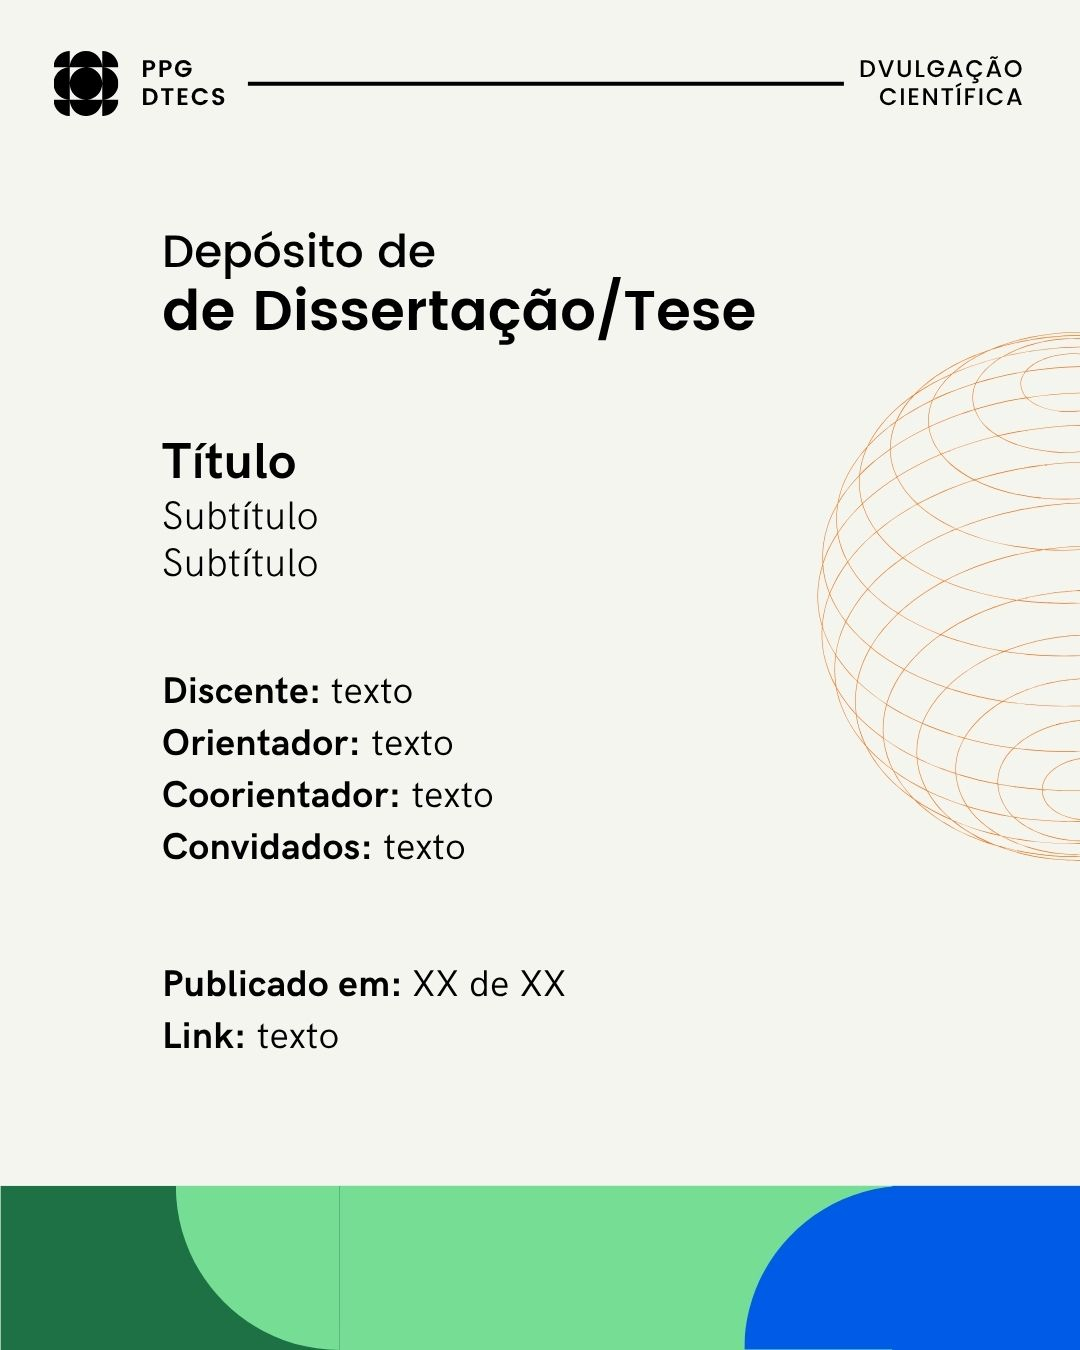
\includegraphics[width=0.5\textwidth]{Figuras/dtecs.jpg}
\caption[Legenda curta de figura]{Legenda mais extensa de figura.}
\label{fig:xwing}
\end{figure}

Dica importante: sempre que possível, use figuras no formato PDF. De acordo com o Overleaf, isso acelera a compilação do texto, sem perder a qualidade da figura. 

\subsection{Exemplo de subseção}\label{subsec:exemploSubsec}
É importante evitar chegar a esse nível de subseção. Dois níveis são suficientes. Use essa opção em último caso, apenas.


\subsection{Exemplo de adição de siglas}\label{subsec:siglas}
Para adicionar uma sigla ou abreviatura na lista de siglas e abreviaturas, use o comando ``\texttt{\textbackslash{}Sigla\{nome por extenso\}\{abreviatura\}}'' ou ``\texttt{\textbackslash{}SiglaHifen\{nome por} \texttt{ex\-ten\-so\}\{abreviatura\}}'' para adicionar a sigla com hífen. 
Por exemplo, respectivamente, \Sigla{Ácido Desoxirribonucleico}{DNA} ou \SiglaHifen{Ácido Ribonucleico}{RNA}. A lista de siglas é adicionada automaticamente.

\section{Comandos opcionais para facilitar}\label{sec:comandosOpc}
Este modelo também criou alguns comandos adicionais não apenas para facilitar o trabalho de quem escreve, mas também para manter uma formatação mais consistente.

Entre esses comandos estão o \texttt{\textbackslash{}ie} que inclui a abreviatura ``\ie'' no texto (equivalente ao ``isto é''). Usar esse comando vai garantir que a abreviatura não se separe entre linhas e que o espaço entre o `.' e a próxima letra seja fixo. O mesmo vale para os comandos \texttt{\textbackslash{}eg} que inclui a abreviatura ``\eg'' e \texttt{\textbackslash{}pex} que inclui a abreviatura ``\pex''.

Também existem os comandos \texttt{\textbackslash{}Capitulo\{rótulo do capítulo\}}, \texttt{\textbackslash{}Equacao\{ró\-tu\-lo da equação\}}, \texttt{\textbackslash{}Figura\{rótulo da figura\}}, \texttt{\textbackslash{}Secao\{rótulo da seção\}} e \texttt{\textbackslash{}Tabela\{rótulo da tabela\}}. Esses comandos inserem referências para os respectivos elementos. Além disso, no próprio texto aparece a \textit{string} (``Capítulo'', ``Equação'', ``Figura'' etc) seguida da referência já com o link. Por exemplo, \Secao{sec:exemplo_secao}. Sugere-se a utilização desses comandos para referenciar os respectivos elementos ao invés do comando \texttt{\textbackslash{}ref\{rótulo\}}. Assim, o texto ficará mais uniforme. 

É possível também usar esses comandos nas versões no plural para conjuntos de referências. Por exemplo, para referenciar várias seções, você pode utilizar o comando \texttt{\textbackslash{}secoes\{ró\-tu\-lo\_1, rótulo\_2, rótulo\_3\}}.

Por exemplo, suponha que queiramos referenciar as \secoes{sec:exemplostabelas,sec:exemplo_secao,subsec:siglas}.
\chapter{Referencial Teórico}\label{chp:Referencial}
% O comando a seguir gera um "dummy text". 
% Elimine-o quando escrever sua dissertação.
\lipsum[6]

\chapter{Metodologia}\label{chp:Metodologia}
% O comando a seguir gera um "dummy text". 
% Elimine-o quando escrever sua dissertação.
\lipsum[7]

\chapter{Resultados}\label{chp:Resultados}
% O comando a seguir gera um "dummy text". 
% Elimine-o quando escrever sua dissertação.
\lipsum[8]
\chapter{Discussão}\label{chp:Discussão}
% O comando a seguir gera um "dummy text". 
% Elimine-o quando escrever sua dissertação.
\lipsum[8]
\chapter{Considerações}\label{chp:Considerações}
% O comando a seguir gera um "dummy text". 
% Elimine-o quando escrever sua dissertação.
\lipsum[8]

% O comando condicional \ifturnitin a seguir é importante para 
% preparar o texto para encaminhamento ao Turnitin. 
% NÃO REMOVA!
% O \fi correspondente está antes do \end{document}
\ifturnitin
    \relax
\else 

%%%%%%%%%%%%%%%%%%%%%%%%%%%%%%%%%%%%%%%%%%%%%%%%%%%%%%%%%%%%%%%%%%
% Elementos pós-textuais
%%%%%%%%%%%%%%%%%%%%%%%%%%%%%%%%%%%%%%%%%%%%%%%%%%%%%%%%%%%%%%%%%%

% Define espaçamento simples em cada referência
\begin{singlespacing}

% Adiciona uma linha em branco entre duas referências
\setlength\bibitemsep{10pt}   
%
% Adiciona as referências bibliográficas.
% Mude o título (title), caso o texto seja em inglês 
% ou espanhol.
\printbibliography[heading=bibintoc, % Adiciona no sumário
                   title={Referências bibliográficas} % Nome do Capítulo
                  ]
\end{singlespacing}

% Os anexos, se houver, vêm depois das referências:
\appendix

% O comando a seguir inclui o arquivo apendices.tex
% que contém os apêndices. Observe o comando \appendix
% na linha anterior
\chapter{Primeiro Apêndice}
% O comando a seguir gera um "dummy text". 
% Elimine-o quando escrever sua dissertação.
\lipsum[9]

\chapter{Segundo  Apêndice}
% O comando a seguir gera um "dummy text". 
% Elimine-o quando escrever sua dissertação.
\lipsum[10]

%
%% O comando \fi a seguir é obrigatório para o controle 
%% da opção "turnitin". Não o remova!
% ... (final do seu documento, apêndices, etc.) ...
\fi % Este é o \fi do bloco do Turnitin

% Exibe a "quarta capa" conhecida como capa de trás
\quartacapa

%%%%%%%%%%%%%%%%%%%%%%%%%%%%%%%%%%%%%%%%%%%%%%%%%%%%%%%%%%%%%%%%%%
\end{document} % Prontinho! Quebre a perna!
%%%%%%%%%%%%%%%%%%%%%%%%%%%%%%%%%%%%%%%%%%%%%%%%%%%%%%%%%%%%%%%%%%